\documentclass[1p]{elsarticle_modified}
%\bibliographystyle{elsarticle-num}

%\usepackage[colorlinks]{hyperref}
%\usepackage{abbrmath_seonhwa} %\Abb, \Ascr, \Acal ,\Abf, \Afrak
\usepackage{amsfonts}
\usepackage{amssymb}
\usepackage{amsmath}
\usepackage{amsthm}
\usepackage{scalefnt}
\usepackage{amsbsy}
\usepackage{kotex}
\usepackage{caption}
\usepackage{subfig}
\usepackage{color}
\usepackage{graphicx}
\usepackage{xcolor} %% white, black, red, green, blue, cyan, magenta, yellow
\usepackage{float}
\usepackage{setspace}
\usepackage{hyperref}

\usepackage{tikz}
\usetikzlibrary{arrows}

\usepackage{multirow}
\usepackage{array} % fixed length table
\usepackage{hhline}

%%%%%%%%%%%%%%%%%%%%%
\makeatletter
\renewcommand*\env@matrix[1][\arraystretch]{%
	\edef\arraystretch{#1}%
	\hskip -\arraycolsep
	\let\@ifnextchar\new@ifnextchar
	\array{*\c@MaxMatrixCols c}}
\makeatother %https://tex.stackexchange.com/questions/14071/how-can-i-increase-the-line-spacing-in-a-matrix
%%%%%%%%%%%%%%%

\usepackage[normalem]{ulem}

\newcommand{\msout}[1]{\ifmmode\text{\sout{\ensuremath{#1}}}\else\sout{#1}\fi}
%SOURCE: \msout is \stkout macro in https://tex.stackexchange.com/questions/20609/strikeout-in-math-mode

\newcommand{\cancel}[1]{
	\ifmmode
	{\color{red}\msout{#1}}
	\else
	{\color{red}\sout{#1}}
	\fi
}

\newcommand{\add}[1]{
	{\color{blue}\uwave{#1}}
}

\newcommand{\replace}[2]{
	\ifmmode
	{\color{red}\msout{#1}}{\color{blue}\uwave{#2}}
	\else
	{\color{red}\sout{#1}}{\color{blue}\uwave{#2}}
	\fi
}

\newcommand{\Sol}{\mathcal{S}} %segment
\newcommand{\D}{D} %diagram
\newcommand{\A}{\mathcal{A}} %arc


%%%%%%%%%%%%%%%%%%%%%%%%%%%%%5 test

\def\sl{\operatorname{\textup{SL}}(2,\Cbb)}
\def\psl{\operatorname{\textup{PSL}}(2,\Cbb)}
\def\quan{\mkern 1mu \triangleright \mkern 1mu}

\theoremstyle{definition}
\newtheorem{thm}{Theorem}[section]
\newtheorem{prop}[thm]{Proposition}
\newtheorem{lem}[thm]{Lemma}
\newtheorem{ques}[thm]{Question}
\newtheorem{cor}[thm]{Corollary}
\newtheorem{defn}[thm]{Definition}
\newtheorem{exam}[thm]{Example}
\newtheorem{rmk}[thm]{Remark}
\newtheorem{alg}[thm]{Algorithm}

\newcommand{\I}{\sqrt{-1}}
\begin{document}

%\begin{frontmatter}
%
%\title{Boundary parabolic representations of knots up to 8 crossings}
%
%%% Group authors per affiliation:
%\author{Yunhi Cho} 
%\address{Department of Mathematics, University of Seoul, Seoul, Korea}
%\ead{yhcho@uos.ac.kr}
%
%
%\author{Seonhwa Kim} %\fnref{s_kim}}
%\address{Center for Geometry and Physics, Institute for Basic Science, Pohang, 37673, Korea}
%\ead{ryeona17@ibs.re.kr}
%
%\author{Hyuk Kim}
%\address{Department of Mathematical Sciences, Seoul National University, Seoul 08826, Korea}
%\ead{hyukkim@snu.ac.kr}
%
%\author{Seokbeom Yoon}
%\address{Department of Mathematical Sciences, Seoul National University, Seoul, 08826,  Korea}
%\ead{sbyoon15@snu.ac.kr}
%
%\begin{abstract}
%We find all boundary parabolic representation of knots up to 8 crossings.
%
%\end{abstract}
%\begin{keyword}
%    \MSC[2010] 57M25 
%\end{keyword}
%
%\end{frontmatter}

%\linenumbers
%\tableofcontents
%
\newcommand\colored[1]{\textcolor{white}{\rule[-0.35ex]{0.8em}{1.4ex}}\kern-0.8em\color{red} #1}%
%\newcommand\colored[1]{\textcolor{white}{ #1}\kern-2.17ex	\textcolor{white}{ #1}\kern-1.81ex	\textcolor{white}{ #1}\kern-2.15ex\color{red}#1	}

{\Large $\underline{12n_{0859}~(K12n_{0859})}$}

\setlength{\tabcolsep}{10pt}
\renewcommand{\arraystretch}{1.6}
\vspace{1cm}\begin{tabular}{m{100pt}>{\centering\arraybackslash}m{274pt}}
\multirow{5}{120pt}{
	\centering
	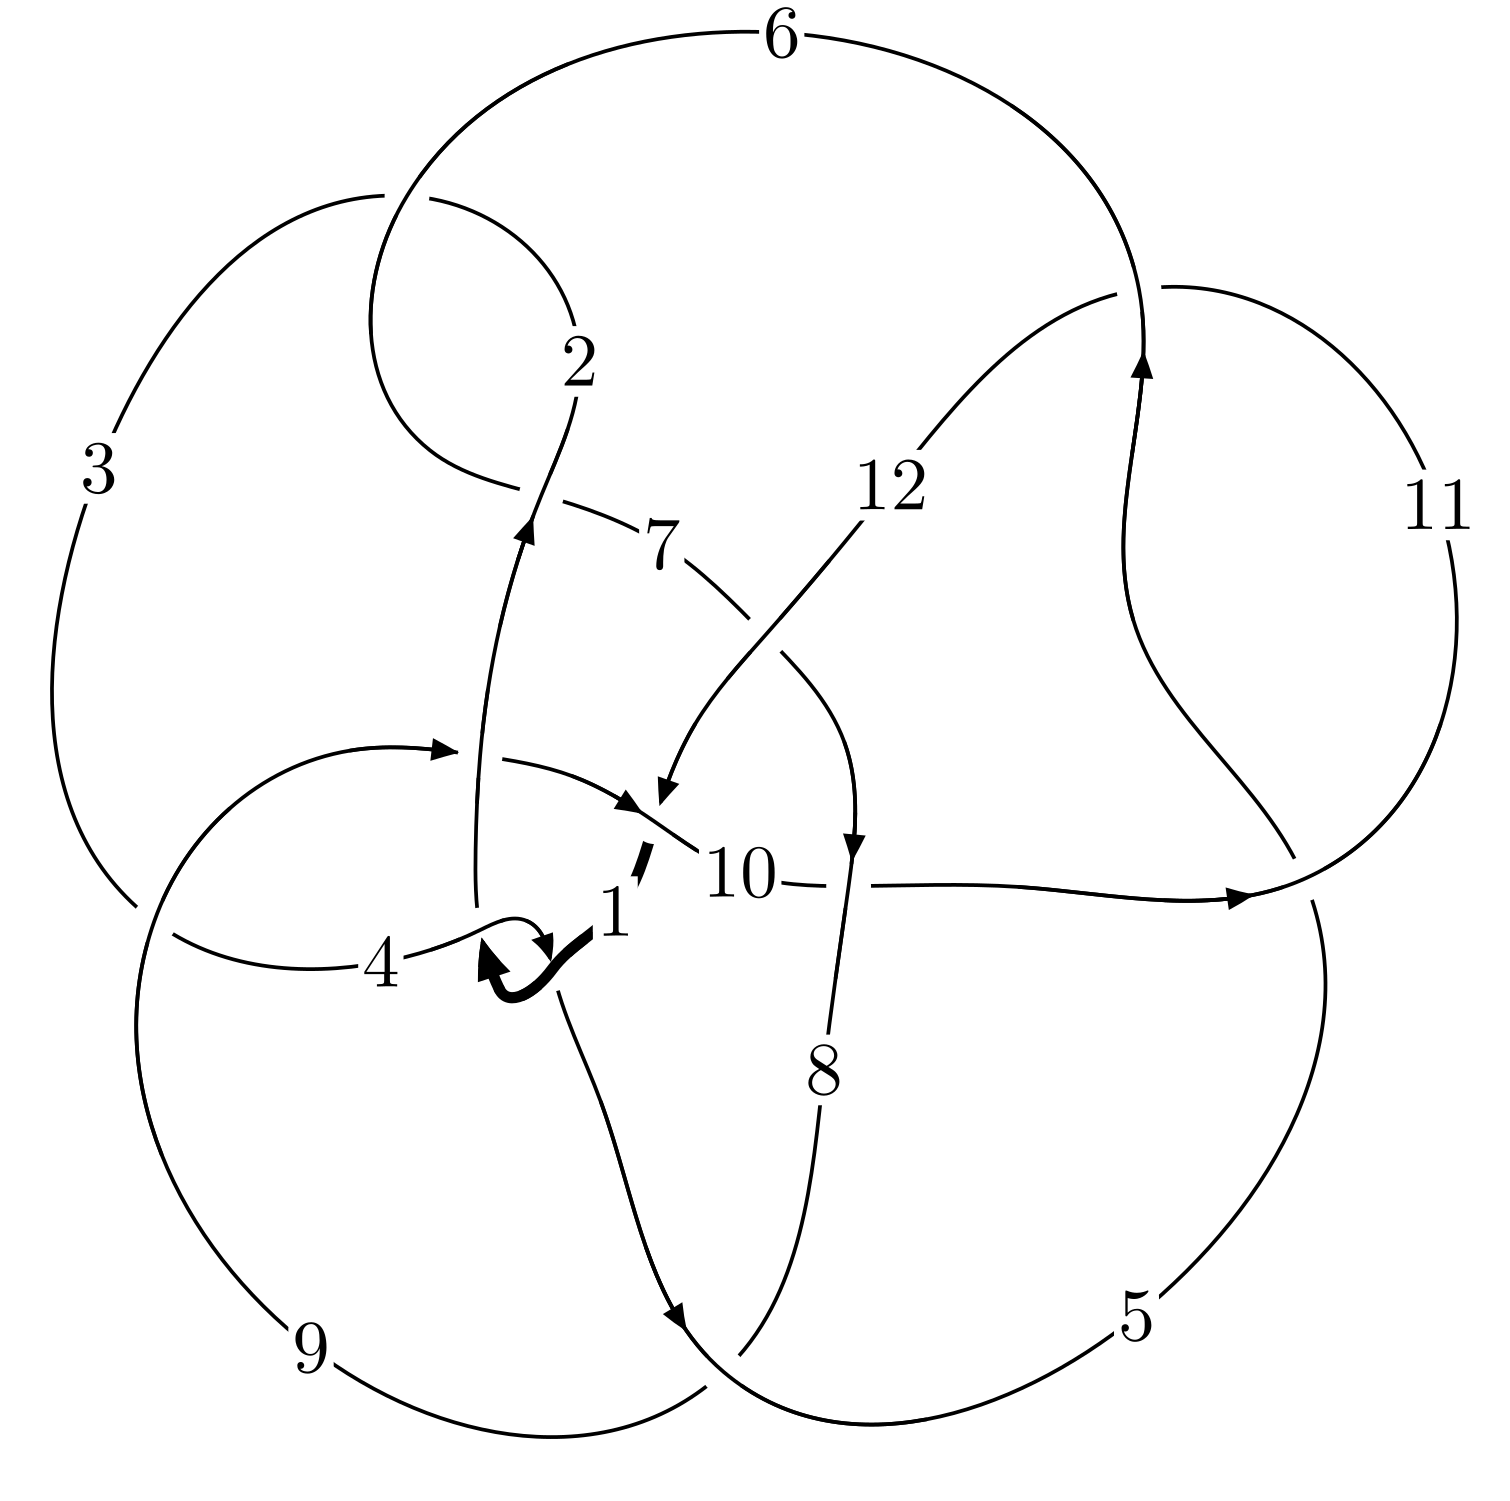
\includegraphics[width=112pt]{../../../GIT/diagram.site/Diagrams/png/2948_12n_0859.png}\\
\ \ \ A knot diagram\footnotemark}&
\allowdisplaybreaks
\textbf{Linearized knot diagam} \\
\cline{2-2}
 &
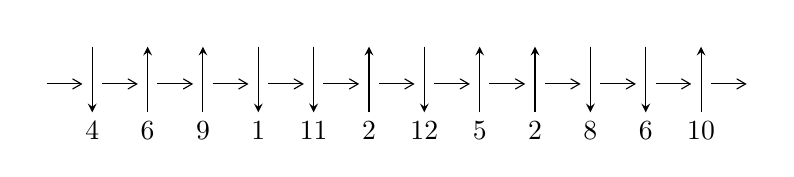
\begin{tikzpicture}[x=20pt, y=17pt]
	% nodes
	\node (C0) at (0, 0) {};
	\node (C1) at (1, 0) {};
	\node (C1U) at (1, +1) {};
	\node (C1D) at (1, -1) {4};

	\node (C2) at (2, 0) {};
	\node (C2U) at (2, +1) {};
	\node (C2D) at (2, -1) {6};

	\node (C3) at (3, 0) {};
	\node (C3U) at (3, +1) {};
	\node (C3D) at (3, -1) {9};

	\node (C4) at (4, 0) {};
	\node (C4U) at (4, +1) {};
	\node (C4D) at (4, -1) {1};

	\node (C5) at (5, 0) {};
	\node (C5U) at (5, +1) {};
	\node (C5D) at (5, -1) {11};

	\node (C6) at (6, 0) {};
	\node (C6U) at (6, +1) {};
	\node (C6D) at (6, -1) {2};

	\node (C7) at (7, 0) {};
	\node (C7U) at (7, +1) {};
	\node (C7D) at (7, -1) {12};

	\node (C8) at (8, 0) {};
	\node (C8U) at (8, +1) {};
	\node (C8D) at (8, -1) {5};

	\node (C9) at (9, 0) {};
	\node (C9U) at (9, +1) {};
	\node (C9D) at (9, -1) {2};

	\node (C10) at (10, 0) {};
	\node (C10U) at (10, +1) {};
	\node (C10D) at (10, -1) {8};

	\node (C11) at (11, 0) {};
	\node (C11U) at (11, +1) {};
	\node (C11D) at (11, -1) {6};

	\node (C12) at (12, 0) {};
	\node (C12U) at (12, +1) {};
	\node (C12D) at (12, -1) {10};
	\node (C13) at (13, 0) {};

	% arrows
	\draw[->,>={angle 60}]
	(C0) edge (C1) (C1) edge (C2) (C2) edge (C3) (C3) edge (C4) (C4) edge (C5) (C5) edge (C6) (C6) edge (C7) (C7) edge (C8) (C8) edge (C9) (C9) edge (C10) (C10) edge (C11) (C11) edge (C12) (C12) edge (C13) ;	\draw[->,>=stealth]
	(C1U) edge (C1D) (C2D) edge (C2U) (C3D) edge (C3U) (C4U) edge (C4D) (C5U) edge (C5D) (C6D) edge (C6U) (C7U) edge (C7D) (C8D) edge (C8U) (C9D) edge (C9U) (C10U) edge (C10D) (C11U) edge (C11D) (C12D) edge (C12U) ;
	\end{tikzpicture} \\
\hhline{~~} \\& 
\textbf{Solving Sequence} \\ \cline{2-2} 
 &
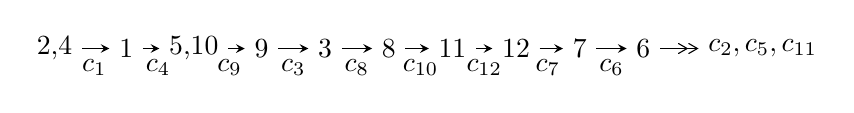
\begin{tikzpicture}[x=23pt, y=7pt]
	% node
	\node (A0) at (-1/8, 0) {2,4};
	\node (A1) at (1, 0) {1};
	\node (A2) at (33/16, 0) {5,10};
	\node (A3) at (25/8, 0) {9};
	\node (A4) at (33/8, 0) {3};
	\node (A5) at (41/8, 0) {8};
	\node (A6) at (49/8, 0) {11};
	\node (A7) at (57/8, 0) {12};
	\node (A8) at (65/8, 0) {7};
	\node (A9) at (73/8, 0) {6};
	\node (C1) at (1/2, -1) {$c_{1}$};
	\node (C2) at (3/2, -1) {$c_{4}$};
	\node (C3) at (21/8, -1) {$c_{9}$};
	\node (C4) at (29/8, -1) {$c_{3}$};
	\node (C5) at (37/8, -1) {$c_{8}$};
	\node (C6) at (45/8, -1) {$c_{10}$};
	\node (C7) at (53/8, -1) {$c_{12}$};
	\node (C8) at (61/8, -1) {$c_{7}$};
	\node (C9) at (69/8, -1) {$c_{6}$};
	\node (A10) at (11, 0) {$c_{2},c_{5},c_{11}$};

	% edge
	\draw[->,>=stealth]	
	(A0) edge (A1) (A1) edge (A2) (A2) edge (A3) (A3) edge (A4) (A4) edge (A5) (A5) edge (A6) (A6) edge (A7) (A7) edge (A8) (A8) edge (A9) ;
	\draw[->>,>={angle 60}]	
	(A9) edge (A10);
\end{tikzpicture} \\ 

\end{tabular} \\

\footnotetext{
The image of knot diagram is generated by the software ``\textbf{Draw programme}" developed by Andrew Bartholomew(\url{http://www.layer8.co.uk/maths/draw/index.htm\#Running-draw}), where we modified some parts for our purpose(\url{https://github.com/CATsTAILs/LinksPainter}).
}\phantom \\ \newline 
\centering \textbf{Ideals for irreducible components\footnotemark of $X_{\text{par}}$} 
 
\begin{align*}
I^u_{1}&=\langle 
2.50974\times10^{289} u^{110}+9.45965\times10^{289} u^{109}+\cdots+4.90170\times10^{288} b+2.02264\times10^{290},\\
\phantom{I^u_{1}}&\phantom{= \langle  }6.11196\times10^{290} u^{110}+2.58646\times10^{291} u^{109}+\cdots+9.31323\times10^{289} a+9.60207\times10^{291},\\
\phantom{I^u_{1}}&\phantom{= \langle  }u^{111}+4 u^{110}+\cdots+75 u+19\rangle \\
I^u_{2}&=\langle 
-6.13493\times10^{24} u^{36}+8.28914\times10^{25} u^{35}+\cdots+1.90673\times10^{25} b+8.11899\times10^{26},\\
\phantom{I^u_{2}}&\phantom{= \langle  }8.06792\times10^{26} u^{36}-5.25168\times10^{27} u^{35}+\cdots+2.09740\times10^{26} a+5.96222\times10^{27},\;u^{37}-7 u^{36}+\cdots-14 u+11\rangle \\
\\
\end{align*}
\raggedright * 2 irreducible components of $\dim_{\mathbb{C}}=0$, with total 148 representations.\\
\footnotetext{All coefficients of polynomials are rational numbers. But the coefficients are sometimes approximated in decimal forms when there is not enough margin.}
\newpage
\renewcommand{\arraystretch}{1}
\centering \section*{I. $I^u_{1}= \langle 2.51\times10^{289} u^{110}+9.46\times10^{289} u^{109}+\cdots+4.90\times10^{288} b+2.02\times10^{290},\;6.11\times10^{290} u^{110}+2.59\times10^{291} u^{109}+\cdots+9.31\times10^{289} a+9.60\times10^{291},\;u^{111}+4 u^{110}+\cdots+75 u+19 \rangle$}
\flushleft \textbf{(i) Arc colorings}\\
\begin{tabular}{m{7pt} m{180pt} m{7pt} m{180pt} }
\flushright $a_{2}=$&$\begin{pmatrix}1\\0\end{pmatrix}$ \\
\flushright $a_{4}=$&$\begin{pmatrix}0\\u\end{pmatrix}$ \\
\flushright $a_{1}=$&$\begin{pmatrix}1\\- u^2\end{pmatrix}$ \\
\flushright $a_{5}=$&$\begin{pmatrix}- u\\u^3+u\end{pmatrix}$ \\
\flushright $a_{10}=$&$\begin{pmatrix}-6.56266 u^{110}-27.7719 u^{109}+\cdots-589.375 u-103.101\\-5.12015 u^{110}-19.2987 u^{109}+\cdots-268.585 u-41.2640\end{pmatrix}$ \\
\flushright $a_{9}=$&$\begin{pmatrix}-1.44251 u^{110}-8.47322 u^{109}+\cdots-320.791 u-61.8374\\-5.12015 u^{110}-19.2987 u^{109}+\cdots-268.585 u-41.2640\end{pmatrix}$ \\
\flushright $a_{3}=$&$\begin{pmatrix}5.94521 u^{110}+22.0082 u^{109}+\cdots+71.6801 u+1.91739\\-1.75109 u^{110}-11.0597 u^{109}+\cdots-474.099 u-132.585\end{pmatrix}$ \\
\flushright $a_{8}=$&$\begin{pmatrix}-4.10108 u^{110}-17.5341 u^{109}+\cdots-396.139 u-56.7976\\-3.25646 u^{110}-11.7527 u^{109}+\cdots-125.743 u-16.4090\end{pmatrix}$ \\
\flushright $a_{11}=$&$\begin{pmatrix}-0.518015 u^{110}-2.04419 u^{109}+\cdots+20.7543 u-8.72507\\3.27484 u^{110}+11.2402 u^{109}+\cdots+20.8357 u-12.9523\end{pmatrix}$ \\
\flushright $a_{12}=$&$\begin{pmatrix}-2.73350 u^{110}-7.81439 u^{109}+\cdots+76.4382 u+41.4901\\-1.58334 u^{110}-5.76715 u^{109}+\cdots-15.7115 u+9.06478\end{pmatrix}$ \\
\flushright $a_{7}=$&$\begin{pmatrix}-2.54528 u^{110}-9.91938 u^{109}+\cdots+58.1041 u+31.4535\\-3.15653 u^{110}-11.4493 u^{109}+\cdots-117.635 u-7.74256\end{pmatrix}$ \\
\flushright $a_{6}=$&$\begin{pmatrix}0.611245 u^{110}+1.52992 u^{109}+\cdots+175.739 u+39.1960\\-3.15653 u^{110}-11.4493 u^{109}+\cdots-117.635 u-7.74256\end{pmatrix}$\\&\end{tabular}
\flushleft \textbf{(ii) Obstruction class $= -1$}\\~\\
\flushleft \textbf{(iii) Cusp Shapes $= 37.2379 u^{110}+165.877 u^{109}+\cdots+3613.83 u+800.617$}\\~\\
\newpage\renewcommand{\arraystretch}{1}
\flushleft \textbf{(iv) u-Polynomials at the component}\newline \\
\begin{tabular}{m{50pt}|m{274pt}}
Crossings & \hspace{64pt}u-Polynomials at each crossing \\
\hline $$\begin{aligned}c_{1},c_{4}\end{aligned}$$&$\begin{aligned}
&u^{111}-4 u^{110}+\cdots+75 u-19
\end{aligned}$\\
\hline $$\begin{aligned}c_{2},c_{6}\end{aligned}$$&$\begin{aligned}
&u^{111}-3 u^{110}+\cdots+11 u+1
\end{aligned}$\\
\hline $$\begin{aligned}c_{3}\end{aligned}$$&$\begin{aligned}
&u^{111}+u^{110}+\cdots-11375608 u+498668
\end{aligned}$\\
\hline $$\begin{aligned}c_{5},c_{11}\end{aligned}$$&$\begin{aligned}
&u^{111}- u^{110}+\cdots+25708 u+2404
\end{aligned}$\\
\hline $$\begin{aligned}c_{7}\end{aligned}$$&$\begin{aligned}
&u^{111}+8 u^{110}+\cdots-3750361 u+280259
\end{aligned}$\\
\hline $$\begin{aligned}c_{8}\end{aligned}$$&$\begin{aligned}
&u^{111}-5 u^{110}+\cdots+1057226 u+206759
\end{aligned}$\\
\hline $$\begin{aligned}c_{9}\end{aligned}$$&$\begin{aligned}
&u^{111}-2 u^{110}+\cdots-11878814 u-708719
\end{aligned}$\\
\hline $$\begin{aligned}c_{10}\end{aligned}$$&$\begin{aligned}
&u^{111}+11 u^{110}+\cdots-13685 u-1355
\end{aligned}$\\
\hline $$\begin{aligned}c_{12}\end{aligned}$$&$\begin{aligned}
&u^{111}+8 u^{110}+\cdots-59598 u-25569
\end{aligned}$\\
\hline
\end{tabular}\\~\\
\newpage\renewcommand{\arraystretch}{1}
\flushleft \textbf{(v) Riley Polynomials at the component}\newline \\
\begin{tabular}{m{50pt}|m{274pt}}
Crossings & \hspace{64pt}Riley Polynomials at each crossing \\
\hline $$\begin{aligned}c_{1},c_{4}\end{aligned}$$&$\begin{aligned}
&y^{111}+68 y^{110}+\cdots-21507 y-361
\end{aligned}$\\
\hline $$\begin{aligned}c_{2},c_{6}\end{aligned}$$&$\begin{aligned}
&y^{111}-75 y^{110}+\cdots-235 y-1
\end{aligned}$\\
\hline $$\begin{aligned}c_{3}\end{aligned}$$&$\begin{aligned}
&y^{111}-15 y^{110}+\cdots+14994491642816 y-248669774224
\end{aligned}$\\
\hline $$\begin{aligned}c_{5},c_{11}\end{aligned}$$&$\begin{aligned}
&y^{111}-61 y^{110}+\cdots+397749808 y-5779216
\end{aligned}$\\
\hline $$\begin{aligned}c_{7}\end{aligned}$$&$\begin{aligned}
&y^{111}+10 y^{110}+\cdots-12572239397577 y-78545107081
\end{aligned}$\\
\hline $$\begin{aligned}c_{8}\end{aligned}$$&$\begin{aligned}
&y^{111}-3 y^{110}+\cdots-601815422274 y-42749284081
\end{aligned}$\\
\hline $$\begin{aligned}c_{9}\end{aligned}$$&$\begin{aligned}
&y^{111}-24 y^{110}+\cdots+75899128605414 y-502282620961
\end{aligned}$\\
\hline $$\begin{aligned}c_{10}\end{aligned}$$&$\begin{aligned}
&y^{111}-41 y^{110}+\cdots+78323675 y-1836025
\end{aligned}$\\
\hline $$\begin{aligned}c_{12}\end{aligned}$$&$\begin{aligned}
&y^{111}-32 y^{110}+\cdots+18684218322 y-653773761
\end{aligned}$\\
\hline
\end{tabular}\\~\\
\newpage\flushleft \textbf{(vi) Complex Volumes and Cusp Shapes}
$$\begin{array}{c|c|c}  
\text{Solutions to }I^u_{1}& \I (\text{vol} + \sqrt{-1}CS) & \text{Cusp shape}\\
 \hline 
\begin{aligned}
u &= -0.275201 + 0.940263 I \\
a &= -1.66878 - 0.15190 I \\
b &= -0.719972 + 0.496650 I\end{aligned}
 & -4.99690 + 6.02322 I & \phantom{-0.000000 } 0 \\ \hline\begin{aligned}
u &= -0.275201 - 0.940263 I \\
a &= -1.66878 + 0.15190 I \\
b &= -0.719972 - 0.496650 I\end{aligned}
 & -4.99690 - 6.02322 I & \phantom{-0.000000 } 0 \\ \hline\begin{aligned}
u &= \phantom{-}0.008257 + 0.975670 I \\
a &= -1.081250 + 0.727074 I \\
b &= -1.054850 - 0.926807 I\end{aligned}
 & \phantom{-}4.64603 + 2.87969 I & \phantom{-0.000000 } 0 \\ \hline\begin{aligned}
u &= \phantom{-}0.008257 - 0.975670 I \\
a &= -1.081250 - 0.727074 I \\
b &= -1.054850 + 0.926807 I\end{aligned}
 & \phantom{-}4.64603 - 2.87969 I & \phantom{-0.000000 } 0 \\ \hline\begin{aligned}
u &= \phantom{-}0.269038 + 0.990512 I \\
a &= \phantom{-}0.06286 - 2.13543 I \\
b &= -0.67117 - 2.58748 I\end{aligned}
 & \phantom{-}1.29416 - 7.64485 I & \phantom{-0.000000 } 0 \\ \hline\begin{aligned}
u &= \phantom{-}0.269038 - 0.990512 I \\
a &= \phantom{-}0.06286 + 2.13543 I \\
b &= -0.67117 + 2.58748 I\end{aligned}
 & \phantom{-}1.29416 + 7.64485 I & \phantom{-0.000000 } 0 \\ \hline\begin{aligned}
u &= \phantom{-}1.015590 + 0.261238 I \\
a &= -0.085276 + 0.232873 I \\
b &= \phantom{-}1.042080 + 0.399877 I\end{aligned}
 & -3.14755 + 4.80636 I & \phantom{-0.000000 } 0 \\ \hline\begin{aligned}
u &= \phantom{-}1.015590 - 0.261238 I \\
a &= -0.085276 - 0.232873 I \\
b &= \phantom{-}1.042080 - 0.399877 I\end{aligned}
 & -3.14755 - 4.80636 I & \phantom{-0.000000 } 0 \\ \hline\begin{aligned}
u &= \phantom{-}0.067968 + 1.053820 I \\
a &= \phantom{-}2.10702 - 1.28713 I \\
b &= \phantom{-}1.159640 - 0.307667 I\end{aligned}
 & \phantom{-}5.06493 - 3.05615 I & \phantom{-0.000000 } 0 \\ \hline\begin{aligned}
u &= \phantom{-}0.067968 - 1.053820 I \\
a &= \phantom{-}2.10702 + 1.28713 I \\
b &= \phantom{-}1.159640 + 0.307667 I\end{aligned}
 & \phantom{-}5.06493 + 3.05615 I & \phantom{-0.000000 } 0\\
 \hline 
 \end{array}$$\newpage$$\begin{array}{c|c|c}  
\text{Solutions to }I^u_{1}& \I (\text{vol} + \sqrt{-1}CS) & \text{Cusp shape}\\
 \hline 
\begin{aligned}
u &= -1.056890 + 0.141190 I \\
a &= -0.169855 + 0.212580 I \\
b &= -1.207740 + 0.615633 I\end{aligned}
 & \phantom{-}3.86792 - 5.81284 I & \phantom{-0.000000 } 0 \\ \hline\begin{aligned}
u &= -1.056890 - 0.141190 I \\
a &= -0.169855 - 0.212580 I \\
b &= -1.207740 - 0.615633 I\end{aligned}
 & \phantom{-}3.86792 + 5.81284 I & \phantom{-0.000000 } 0 \\ \hline\begin{aligned}
u &= -0.203436 + 0.909772 I \\
a &= \phantom{-}1.307750 - 0.110479 I \\
b &= \phantom{-}0.638602 - 0.771746 I\end{aligned}
 & \phantom{-}0.60675 + 2.77436 I & \phantom{-0.000000 } 0 \\ \hline\begin{aligned}
u &= -0.203436 - 0.909772 I \\
a &= \phantom{-}1.307750 + 0.110479 I \\
b &= \phantom{-}0.638602 + 0.771746 I\end{aligned}
 & \phantom{-}0.60675 - 2.77436 I & \phantom{-0.000000 } 0 \\ \hline\begin{aligned}
u &= \phantom{-}0.273074 + 0.880594 I \\
a &= -1.15007 + 1.36087 I \\
b &= -0.49476 + 2.05464 I\end{aligned}
 & \phantom{-}2.04876 - 2.43910 I & \phantom{-0.000000 } 0 \\ \hline\begin{aligned}
u &= \phantom{-}0.273074 - 0.880594 I \\
a &= -1.15007 - 1.36087 I \\
b &= -0.49476 - 2.05464 I\end{aligned}
 & \phantom{-}2.04876 + 2.43910 I & \phantom{-0.000000 } 0 \\ \hline\begin{aligned}
u &= \phantom{-}0.944619 + 0.528913 I \\
a &= -0.242883 - 0.203509 I \\
b &= -0.722055 + 0.054677 I\end{aligned}
 & -0.771420 - 0.536538 I & \phantom{-0.000000 } 0 \\ \hline\begin{aligned}
u &= \phantom{-}0.944619 - 0.528913 I \\
a &= -0.242883 + 0.203509 I \\
b &= -0.722055 - 0.054677 I\end{aligned}
 & -0.771420 + 0.536538 I & \phantom{-0.000000 } 0 \\ \hline\begin{aligned}
u &= -1.078500 + 0.127411 I \\
a &= -0.0065061 - 0.1213240 I \\
b &= \phantom{-}1.16595 - 0.88431 I\end{aligned}
 & \phantom{-}0.42740 - 12.79140 I & \phantom{-0.000000 } 0 \\ \hline\begin{aligned}
u &= -1.078500 - 0.127411 I \\
a &= -0.0065061 + 0.1213240 I \\
b &= \phantom{-}1.16595 + 0.88431 I\end{aligned}
 & \phantom{-}0.42740 + 12.79140 I & \phantom{-0.000000 } 0\\
 \hline 
 \end{array}$$\newpage$$\begin{array}{c|c|c}  
\text{Solutions to }I^u_{1}& \I (\text{vol} + \sqrt{-1}CS) & \text{Cusp shape}\\
 \hline 
\begin{aligned}
u &= \phantom{-}0.236625 + 0.869701 I \\
a &= -3.32187 - 0.04411 I \\
b &= -0.121924 + 0.748351 I\end{aligned}
 & \phantom{-}0.42650 - 6.83508 I & \phantom{-0.000000 } 0 \\ \hline\begin{aligned}
u &= \phantom{-}0.236625 - 0.869701 I \\
a &= -3.32187 + 0.04411 I \\
b &= -0.121924 - 0.748351 I\end{aligned}
 & \phantom{-}0.42650 + 6.83508 I & \phantom{-0.000000 } 0 \\ \hline\begin{aligned}
u &= -0.461544 + 0.772795 I \\
a &= -1.49141 + 1.22164 I \\
b &= -1.53587 + 0.71027 I\end{aligned}
 & \phantom{-}0.82911 - 1.58249 I & \phantom{-0.000000 } 0 \\ \hline\begin{aligned}
u &= -0.461544 - 0.772795 I \\
a &= -1.49141 - 1.22164 I \\
b &= -1.53587 - 0.71027 I\end{aligned}
 & \phantom{-}0.82911 + 1.58249 I & \phantom{-0.000000 } 0 \\ \hline\begin{aligned}
u &= \phantom{-}0.713611 + 0.529292 I \\
a &= \phantom{-}0.585808 + 0.306800 I \\
b &= \phantom{-}0.259462 - 0.808596 I\end{aligned}
 & -5.15394 - 2.61216 I & \phantom{-0.000000 } 0 \\ \hline\begin{aligned}
u &= \phantom{-}0.713611 - 0.529292 I \\
a &= \phantom{-}0.585808 - 0.306800 I \\
b &= \phantom{-}0.259462 + 0.808596 I\end{aligned}
 & -5.15394 + 2.61216 I & \phantom{-0.000000 } 0 \\ \hline\begin{aligned}
u &= \phantom{-}1.110890 + 0.069837 I \\
a &= \phantom{-}0.0652080 + 0.0323979 I \\
b &= \phantom{-}0.107631 + 1.122940 I\end{aligned}
 & -5.70817 - 1.45948 I & \phantom{-0.000000 } 0 \\ \hline\begin{aligned}
u &= \phantom{-}1.110890 - 0.069837 I \\
a &= \phantom{-}0.0652080 - 0.0323979 I \\
b &= \phantom{-}0.107631 - 1.122940 I\end{aligned}
 & -5.70817 + 1.45948 I & \phantom{-0.000000 } 0 \\ \hline\begin{aligned}
u &= -0.237461 + 0.845090 I \\
a &= \phantom{-}2.16570 + 1.55417 I \\
b &= \phantom{-}0.64302 + 2.18678 I\end{aligned}
 & -5.57793 + 1.17653 I & \phantom{-0.000000 } 0 \\ \hline\begin{aligned}
u &= -0.237461 - 0.845090 I \\
a &= \phantom{-}2.16570 - 1.55417 I \\
b &= \phantom{-}0.64302 - 2.18678 I\end{aligned}
 & -5.57793 - 1.17653 I & \phantom{-0.000000 } 0\\
 \hline 
 \end{array}$$\newpage$$\begin{array}{c|c|c}  
\text{Solutions to }I^u_{1}& \I (\text{vol} + \sqrt{-1}CS) & \text{Cusp shape}\\
 \hline 
\begin{aligned}
u &= -0.338976 + 0.788941 I \\
a &= -1.97899 - 0.01191 I \\
b &= -0.135954 - 1.404000 I\end{aligned}
 & -6.29732 + 1.56335 I & \phantom{-0.000000 } 0 \\ \hline\begin{aligned}
u &= -0.338976 - 0.788941 I \\
a &= -1.97899 + 0.01191 I \\
b &= -0.135954 + 1.404000 I\end{aligned}
 & -6.29732 - 1.56335 I & \phantom{-0.000000 } 0 \\ \hline\begin{aligned}
u &= -0.671253 + 0.522611 I \\
a &= -0.898132 - 0.522684 I \\
b &= \phantom{-}0.750246 + 0.666293 I\end{aligned}
 & \phantom{-}1.17995 + 3.44561 I & \phantom{-0.000000 } 0 \\ \hline\begin{aligned}
u &= -0.671253 - 0.522611 I \\
a &= -0.898132 + 0.522684 I \\
b &= \phantom{-}0.750246 - 0.666293 I\end{aligned}
 & \phantom{-}1.17995 - 3.44561 I & \phantom{-0.000000 } 0 \\ \hline\begin{aligned}
u &= -0.839318 + 0.060783 I \\
a &= \phantom{-}0.493485 + 0.050564 I \\
b &= \phantom{-}0.607833 - 0.088103 I\end{aligned}
 & -3.61948 + 0.00513 I & \phantom{-0.000000 } 0 \\ \hline\begin{aligned}
u &= -0.839318 - 0.060783 I \\
a &= \phantom{-}0.493485 - 0.050564 I \\
b &= \phantom{-}0.607833 + 0.088103 I\end{aligned}
 & -3.61948 - 0.00513 I & \phantom{-0.000000 } 0 \\ \hline\begin{aligned}
u &= \phantom{-}0.262200 + 1.137650 I \\
a &= \phantom{-}1.99952 - 0.20662 I \\
b &= \phantom{-}0.880763 - 0.924406 I\end{aligned}
 & \phantom{-}4.21579 - 3.30687 I & \phantom{-0.000000 } 0 \\ \hline\begin{aligned}
u &= \phantom{-}0.262200 - 1.137650 I \\
a &= \phantom{-}1.99952 + 0.20662 I \\
b &= \phantom{-}0.880763 + 0.924406 I\end{aligned}
 & \phantom{-}4.21579 + 3.30687 I & \phantom{-0.000000 } 0 \\ \hline\begin{aligned}
u &= -0.831831 + 0.026807 I \\
a &= -0.446008 - 0.058527 I \\
b &= \phantom{-}1.155800 + 0.449895 I\end{aligned}
 & \phantom{-}4.08247 + 1.05839 I & \phantom{-0.000000 } 0 \\ \hline\begin{aligned}
u &= -0.831831 - 0.026807 I \\
a &= -0.446008 + 0.058527 I \\
b &= \phantom{-}1.155800 - 0.449895 I\end{aligned}
 & \phantom{-}4.08247 - 1.05839 I & \phantom{-0.000000 } 0\\
 \hline 
 \end{array}$$\newpage$$\begin{array}{c|c|c}  
\text{Solutions to }I^u_{1}& \I (\text{vol} + \sqrt{-1}CS) & \text{Cusp shape}\\
 \hline 
\begin{aligned}
u &= -0.447141 + 1.081630 I \\
a &= \phantom{-}0.61140 - 1.30410 I \\
b &= \phantom{-}1.151160 - 0.361627 I\end{aligned}
 & \phantom{-}5.88221 - 1.78475 I & \phantom{-0.000000 } 0 \\ \hline\begin{aligned}
u &= -0.447141 - 1.081630 I \\
a &= \phantom{-}0.61140 + 1.30410 I \\
b &= \phantom{-}1.151160 + 0.361627 I\end{aligned}
 & \phantom{-}5.88221 + 1.78475 I & \phantom{-0.000000 } 0 \\ \hline\begin{aligned}
u &= -0.444421 + 0.660349 I \\
a &= \phantom{-}1.349300 + 0.372347 I \\
b &= -0.593114 - 0.380848 I\end{aligned}
 & \phantom{-}1.50618 + 1.02895 I & \phantom{-0.000000 } 0 \\ \hline\begin{aligned}
u &= -0.444421 - 0.660349 I \\
a &= \phantom{-}1.349300 - 0.372347 I \\
b &= -0.593114 + 0.380848 I\end{aligned}
 & \phantom{-}1.50618 - 1.02895 I & \phantom{-0.000000 } 0 \\ \hline\begin{aligned}
u &= \phantom{-}0.314688 + 0.716816 I \\
a &= -1.07783 - 1.35538 I \\
b &= \phantom{-}0.211726 + 1.211480 I\end{aligned}
 & \phantom{-}0.13373 + 4.14099 I & \phantom{-0.000000 } 0 \\ \hline\begin{aligned}
u &= \phantom{-}0.314688 - 0.716816 I \\
a &= -1.07783 + 1.35538 I \\
b &= \phantom{-}0.211726 - 1.211480 I\end{aligned}
 & \phantom{-}0.13373 - 4.14099 I & \phantom{-0.000000 } 0 \\ \hline\begin{aligned}
u &= \phantom{-}0.551417 + 1.086260 I \\
a &= \phantom{-}0.368193 - 0.274729 I \\
b &= -0.037286 + 0.326195 I\end{aligned}
 & -1.74777 - 5.52938 I & \phantom{-0.000000 } 0 \\ \hline\begin{aligned}
u &= \phantom{-}0.551417 - 1.086260 I \\
a &= \phantom{-}0.368193 + 0.274729 I \\
b &= -0.037286 - 0.326195 I\end{aligned}
 & -1.74777 + 5.52938 I & \phantom{-0.000000 } 0 \\ \hline\begin{aligned}
u &= -0.259852 + 1.193850 I \\
a &= -1.37826 + 1.79128 I \\
b &= -0.760498 - 0.282882 I\end{aligned}
 & \phantom{-}3.97987 + 7.49973 I & \phantom{-0.000000 } 0 \\ \hline\begin{aligned}
u &= -0.259852 - 1.193850 I \\
a &= -1.37826 - 1.79128 I \\
b &= -0.760498 + 0.282882 I\end{aligned}
 & \phantom{-}3.97987 - 7.49973 I & \phantom{-0.000000 } 0\\
 \hline 
 \end{array}$$\newpage$$\begin{array}{c|c|c}  
\text{Solutions to }I^u_{1}& \I (\text{vol} + \sqrt{-1}CS) & \text{Cusp shape}\\
 \hline 
\begin{aligned}
u &= \phantom{-}0.445330 + 1.139830 I \\
a &= -1.045090 - 0.267342 I \\
b &= -1.102600 - 0.164427 I\end{aligned}
 & -1.16332 - 3.35103 I & \phantom{-0.000000 } 0 \\ \hline\begin{aligned}
u &= \phantom{-}0.445330 - 1.139830 I \\
a &= -1.045090 + 0.267342 I \\
b &= -1.102600 + 0.164427 I\end{aligned}
 & -1.16332 + 3.35103 I & \phantom{-0.000000 } 0 \\ \hline\begin{aligned}
u &= -0.100145 + 0.768474 I \\
a &= -1.46998 - 0.05204 I \\
b &= -0.736228 + 0.492817 I\end{aligned}
 & \phantom{-}0.045168 - 0.756689 I & \phantom{-0.000000 } 0 \\ \hline\begin{aligned}
u &= -0.100145 - 0.768474 I \\
a &= -1.46998 + 0.05204 I \\
b &= -0.736228 - 0.492817 I\end{aligned}
 & \phantom{-}0.045168 + 0.756689 I & \phantom{-0.000000 } 0 \\ \hline\begin{aligned}
u &= \phantom{-}0.293488 + 1.192270 I \\
a &= \phantom{-}1.69050 + 0.02346 I \\
b &= \phantom{-}0.972454 - 0.865758 I\end{aligned}
 & \phantom{-}4.19599 - 3.22298 I & \phantom{-0.000000 } 0 \\ \hline\begin{aligned}
u &= \phantom{-}0.293488 - 1.192270 I \\
a &= \phantom{-}1.69050 - 0.02346 I \\
b &= \phantom{-}0.972454 + 0.865758 I\end{aligned}
 & \phantom{-}4.19599 + 3.22298 I & \phantom{-0.000000 } 0 \\ \hline\begin{aligned}
u &= -0.280377 + 1.214070 I \\
a &= \phantom{-}2.09638 + 0.11720 I \\
b &= \phantom{-}2.00898 + 0.67625 I\end{aligned}
 & \phantom{-}5.90966 + 3.14124 I & \phantom{-0.000000 } 0 \\ \hline\begin{aligned}
u &= -0.280377 - 1.214070 I \\
a &= \phantom{-}2.09638 - 0.11720 I \\
b &= \phantom{-}2.00898 - 0.67625 I\end{aligned}
 & \phantom{-}5.90966 - 3.14124 I & \phantom{-0.000000 } 0 \\ \hline\begin{aligned}
u &= -0.737383 + 0.092217 I \\
a &= \phantom{-}0.259636 - 0.112181 I \\
b &= -1.080860 + 0.872100 I\end{aligned}
 & \phantom{-}2.57136 - 5.52359 I & \phantom{-0.000000 } 0 \\ \hline\begin{aligned}
u &= -0.737383 - 0.092217 I \\
a &= \phantom{-}0.259636 + 0.112181 I \\
b &= -1.080860 - 0.872100 I\end{aligned}
 & \phantom{-}2.57136 + 5.52359 I & \phantom{-0.000000 } 0\\
 \hline 
 \end{array}$$\newpage$$\begin{array}{c|c|c}  
\text{Solutions to }I^u_{1}& \I (\text{vol} + \sqrt{-1}CS) & \text{Cusp shape}\\
 \hline 
\begin{aligned}
u &= \phantom{-}0.738210 + 0.077832 I \\
a &= -0.410329 - 0.870145 I \\
b &= \phantom{-}0.416517 - 0.282826 I\end{aligned}
 & -4.53991 + 0.81092 I & \phantom{-0.000000 } 0 \\ \hline\begin{aligned}
u &= \phantom{-}0.738210 - 0.077832 I \\
a &= -0.410329 + 0.870145 I \\
b &= \phantom{-}0.416517 + 0.282826 I\end{aligned}
 & -4.53991 - 0.81092 I & \phantom{-0.000000 } 0 \\ \hline\begin{aligned}
u &= -0.459139 + 1.195040 I \\
a &= \phantom{-}2.01127 - 0.25782 I \\
b &= \phantom{-}1.43948 + 1.12235 I\end{aligned}
 & \phantom{-}5.82742 + 9.96822 I & \phantom{-0.000000 } 0 \\ \hline\begin{aligned}
u &= -0.459139 - 1.195040 I \\
a &= \phantom{-}2.01127 + 0.25782 I \\
b &= \phantom{-}1.43948 - 1.12235 I\end{aligned}
 & \phantom{-}5.82742 - 9.96822 I & \phantom{-0.000000 } 0 \\ \hline\begin{aligned}
u &= -1.29696\phantom{ +0.000000I} \\
a &= \phantom{-}0.254156\phantom{ +0.000000I} \\
b &= -0.605822\phantom{ +0.000000I}\end{aligned}
 & -2.36547\phantom{ +0.000000I} & \phantom{-0.000000 } 0 \\ \hline\begin{aligned}
u &= \phantom{-}0.408571 + 0.565367 I \\
a &= -1.92263 + 0.91363 I \\
b &= -0.50537 + 1.33287 I\end{aligned}
 & \phantom{-}1.35718 - 0.65015 I & \phantom{-0.000000 } 0 \\ \hline\begin{aligned}
u &= \phantom{-}0.408571 - 0.565367 I \\
a &= -1.92263 - 0.91363 I \\
b &= -0.50537 - 1.33287 I\end{aligned}
 & \phantom{-}1.35718 + 0.65015 I & \phantom{-0.000000 } 0 \\ \hline\begin{aligned}
u &= \phantom{-}0.275750 + 1.281120 I \\
a &= -1.267620 - 0.360467 I \\
b &= -1.164700 + 0.486012 I\end{aligned}
 & \phantom{-}2.25301 + 0.74215 I & \phantom{-0.000000 } 0 \\ \hline\begin{aligned}
u &= \phantom{-}0.275750 - 1.281120 I \\
a &= -1.267620 + 0.360467 I \\
b &= -1.164700 - 0.486012 I\end{aligned}
 & \phantom{-}2.25301 - 0.74215 I & \phantom{-0.000000 } 0 \\ \hline\begin{aligned}
u &= -0.509886 + 1.209580 I \\
a &= -0.968689 + 0.852632 I \\
b &= -1.40376 - 0.22411 I\end{aligned}
 & \phantom{-}7.48694 + 3.68062 I & \phantom{-0.000000 } 0\\
 \hline 
 \end{array}$$\newpage$$\begin{array}{c|c|c}  
\text{Solutions to }I^u_{1}& \I (\text{vol} + \sqrt{-1}CS) & \text{Cusp shape}\\
 \hline 
\begin{aligned}
u &= -0.509886 - 1.209580 I \\
a &= -0.968689 - 0.852632 I \\
b &= -1.40376 + 0.22411 I\end{aligned}
 & \phantom{-}7.48694 - 3.68062 I & \phantom{-0.000000 } 0 \\ \hline\begin{aligned}
u &= -0.280540 + 0.626809 I \\
a &= \phantom{-}1.72125 + 0.36677 I \\
b &= \phantom{-}0.604732 - 0.417904 I\end{aligned}
 & -5.87578 - 3.33399 I & \phantom{-0.000000 } 0 \\ \hline\begin{aligned}
u &= -0.280540 - 0.626809 I \\
a &= \phantom{-}1.72125 - 0.36677 I \\
b &= \phantom{-}0.604732 + 0.417904 I\end{aligned}
 & -5.87578 + 3.33399 I & \phantom{-0.000000 } 0 \\ \hline\begin{aligned}
u &= \phantom{-}0.332184 + 1.282280 I \\
a &= -1.144800 + 0.071823 I \\
b &= -0.591057 + 0.882017 I\end{aligned}
 & \phantom{-}0.02593 - 6.00299 I & \phantom{-0.000000 } 0 \\ \hline\begin{aligned}
u &= \phantom{-}0.332184 - 1.282280 I \\
a &= -1.144800 - 0.071823 I \\
b &= -0.591057 - 0.882017 I\end{aligned}
 & \phantom{-}0.02593 + 6.00299 I & \phantom{-0.000000 } 0 \\ \hline\begin{aligned}
u &= -0.448427 + 1.254430 I \\
a &= -1.72331 + 0.34160 I \\
b &= -1.64583 - 0.95608 I\end{aligned}
 & \phantom{-}7.92858 + 5.65757 I & \phantom{-0.000000 } 0 \\ \hline\begin{aligned}
u &= -0.448427 - 1.254430 I \\
a &= -1.72331 - 0.34160 I \\
b &= -1.64583 + 0.95608 I\end{aligned}
 & \phantom{-}7.92858 - 5.65757 I & \phantom{-0.000000 } 0 \\ \hline\begin{aligned}
u &= \phantom{-}0.649724 + 1.209040 I \\
a &= \phantom{-}0.934100 + 0.639804 I \\
b &= \phantom{-}1.109860 - 0.186332 I\end{aligned}
 & \phantom{-}1.52430 - 5.45836 I & \phantom{-0.000000 } 0 \\ \hline\begin{aligned}
u &= \phantom{-}0.649724 - 1.209040 I \\
a &= \phantom{-}0.934100 - 0.639804 I \\
b &= \phantom{-}1.109860 + 0.186332 I\end{aligned}
 & \phantom{-}1.52430 + 5.45836 I & \phantom{-0.000000 } 0 \\ \hline\begin{aligned}
u &= -0.319391 + 1.343010 I \\
a &= -1.62626 - 0.38363 I \\
b &= -1.73839 - 1.28747 I\end{aligned}
 & \phantom{-}6.78734 + 6.74957 I & \phantom{-0.000000 } 0\\
 \hline 
 \end{array}$$\newpage$$\begin{array}{c|c|c}  
\text{Solutions to }I^u_{1}& \I (\text{vol} + \sqrt{-1}CS) & \text{Cusp shape}\\
 \hline 
\begin{aligned}
u &= -0.319391 - 1.343010 I \\
a &= -1.62626 + 0.38363 I \\
b &= -1.73839 + 1.28747 I\end{aligned}
 & \phantom{-}6.78734 - 6.74957 I & \phantom{-0.000000 } 0 \\ \hline\begin{aligned}
u &= \phantom{-}0.595501 + 1.255810 I \\
a &= -1.43242 - 0.50104 I \\
b &= -1.46776 + 0.72438 I\end{aligned}
 & -0.01416 - 10.61690 I & \phantom{-0.000000 } 0 \\ \hline\begin{aligned}
u &= \phantom{-}0.595501 - 1.255810 I \\
a &= -1.43242 + 0.50104 I \\
b &= -1.46776 - 0.72438 I\end{aligned}
 & -0.01416 + 10.61690 I & \phantom{-0.000000 } 0 \\ \hline\begin{aligned}
u &= -0.519632 + 1.303580 I \\
a &= -1.51849 + 0.52896 I \\
b &= -1.172690 - 0.361484 I\end{aligned}
 & \phantom{-}0.19967 + 5.22519 I & \phantom{-0.000000 } 0 \\ \hline\begin{aligned}
u &= -0.519632 - 1.303580 I \\
a &= -1.51849 - 0.52896 I \\
b &= -1.172690 + 0.361484 I\end{aligned}
 & \phantom{-}0.19967 - 5.22519 I & \phantom{-0.000000 } 0 \\ \hline\begin{aligned}
u &= -0.57152 + 1.29938 I \\
a &= \phantom{-}1.76760 - 0.41531 I \\
b &= \phantom{-}1.57268 + 0.78579 I\end{aligned}
 & \phantom{-}7.48757 + 11.61040 I & \phantom{-0.000000 } 0 \\ \hline\begin{aligned}
u &= -0.57152 - 1.29938 I \\
a &= \phantom{-}1.76760 + 0.41531 I \\
b &= \phantom{-}1.57268 - 0.78579 I\end{aligned}
 & \phantom{-}7.48757 - 11.61040 I & \phantom{-0.000000 } 0 \\ \hline\begin{aligned}
u &= \phantom{-}0.57393 + 1.30349 I \\
a &= -1.258510 + 0.260259 I \\
b &= -0.642563 + 1.019860 I\end{aligned}
 & -1.91021 - 4.45206 I & \phantom{-0.000000 } 0 \\ \hline\begin{aligned}
u &= \phantom{-}0.57393 - 1.30349 I \\
a &= -1.258510 - 0.260259 I \\
b &= -0.642563 - 1.019860 I\end{aligned}
 & -1.91021 + 4.45206 I & \phantom{-0.000000 } 0 \\ \hline\begin{aligned}
u &= -0.57654 + 1.30702 I \\
a &= -1.79727 + 0.24737 I \\
b &= -1.51657 - 1.11069 I\end{aligned}
 & \phantom{-}4.1086 + 18.6576 I & \phantom{-0.000000 } 0\\
 \hline 
 \end{array}$$\newpage$$\begin{array}{c|c|c}  
\text{Solutions to }I^u_{1}& \I (\text{vol} + \sqrt{-1}CS) & \text{Cusp shape}\\
 \hline 
\begin{aligned}
u &= -0.57654 - 1.30702 I \\
a &= -1.79727 - 0.24737 I \\
b &= -1.51657 + 1.11069 I\end{aligned}
 & \phantom{-}4.1086 - 18.6576 I & \phantom{-0.000000 } 0 \\ \hline\begin{aligned}
u &= -0.36392 + 1.39393 I \\
a &= \phantom{-}1.080680 - 0.889817 I \\
b &= \phantom{-}1.094080 - 0.092347 I\end{aligned}
 & \phantom{-}8.99561 - 0.74820 I & \phantom{-0.000000 } 0 \\ \hline\begin{aligned}
u &= -0.36392 - 1.39393 I \\
a &= \phantom{-}1.080680 + 0.889817 I \\
b &= \phantom{-}1.094080 + 0.092347 I\end{aligned}
 & \phantom{-}8.99561 + 0.74820 I & \phantom{-0.000000 } 0 \\ \hline\begin{aligned}
u &= \phantom{-}0.094811 + 0.549038 I \\
a &= \phantom{-}3.77075 - 1.38548 I \\
b &= \phantom{-}1.52223 - 1.11379 I\end{aligned}
 & -0.07750 + 5.29942 I & -5.40871 - 2.98457 I \\ \hline\begin{aligned}
u &= \phantom{-}0.094811 - 0.549038 I \\
a &= \phantom{-}3.77075 + 1.38548 I \\
b &= \phantom{-}1.52223 + 1.11379 I\end{aligned}
 & -0.07750 - 5.29942 I & -5.40871 + 2.98457 I \\ \hline\begin{aligned}
u &= -0.03969 + 1.44624 I \\
a &= \phantom{-}1.81423 - 0.86290 I \\
b &= \phantom{-}0.810507 - 0.314287 I\end{aligned}
 & \phantom{-}7.88736 - 1.01294 I & \phantom{-0.000000 } 0 \\ \hline\begin{aligned}
u &= -0.03969 - 1.44624 I \\
a &= \phantom{-}1.81423 + 0.86290 I \\
b &= \phantom{-}0.810507 + 0.314287 I\end{aligned}
 & \phantom{-}7.88736 + 1.01294 I & \phantom{-0.000000 } 0 \\ \hline\begin{aligned}
u &= -0.346914 + 0.399228 I \\
a &= \phantom{-}2.09323 - 2.49228 I \\
b &= \phantom{-}1.47129 - 0.39004 I\end{aligned}
 & \phantom{-}0.02497 + 5.27393 I & -3.58834 - 5.27961 I \\ \hline\begin{aligned}
u &= -0.346914 - 0.399228 I \\
a &= \phantom{-}2.09323 + 2.49228 I \\
b &= \phantom{-}1.47129 + 0.39004 I\end{aligned}
 & \phantom{-}0.02497 - 5.27393 I & -3.58834 + 5.27961 I \\ \hline\begin{aligned}
u &= -0.37718 + 1.44983 I \\
a &= -0.716966 + 0.800137 I \\
b &= -1.076310 + 0.259767 I\end{aligned}
 & \phantom{-}5.63085 - 7.45344 I & \phantom{-0.000000 } 0\\
 \hline 
 \end{array}$$\newpage$$\begin{array}{c|c|c}  
\text{Solutions to }I^u_{1}& \I (\text{vol} + \sqrt{-1}CS) & \text{Cusp shape}\\
 \hline 
\begin{aligned}
u &= -0.37718 - 1.44983 I \\
a &= -0.716966 - 0.800137 I \\
b &= -1.076310 - 0.259767 I\end{aligned}
 & \phantom{-}5.63085 + 7.45344 I & \phantom{-0.000000 } 0 \\ \hline\begin{aligned}
u &= \phantom{-}0.57631 + 1.39320 I \\
a &= \phantom{-}0.935947 - 0.425096 I \\
b &= \phantom{-}0.472657 - 1.103060 I\end{aligned}
 & -1.17664 - 7.45881 I & \phantom{-0.000000 } 0 \\ \hline\begin{aligned}
u &= \phantom{-}0.57631 - 1.39320 I \\
a &= \phantom{-}0.935947 + 0.425096 I \\
b &= \phantom{-}0.472657 + 1.103060 I\end{aligned}
 & -1.17664 + 7.45881 I & \phantom{-0.000000 } 0 \\ \hline\begin{aligned}
u &= -0.63748 + 1.37589 I \\
a &= \phantom{-}0.701318 - 0.217635 I \\
b &= \phantom{-}0.925253 + 0.716207 I\end{aligned}
 & \phantom{-}1.91629 + 6.72215 I & \phantom{-0.000000 } 0 \\ \hline\begin{aligned}
u &= -0.63748 - 1.37589 I \\
a &= \phantom{-}0.701318 + 0.217635 I \\
b &= \phantom{-}0.925253 - 0.716207 I\end{aligned}
 & \phantom{-}1.91629 - 6.72215 I & \phantom{-0.000000 } 0 \\ \hline\begin{aligned}
u &= \phantom{-}0.186229 + 0.352117 I \\
a &= -0.996682 - 0.693951 I \\
b &= -0.390010 + 0.415908 I\end{aligned}
 & \phantom{-}0.019457 - 0.961906 I & \phantom{-}0.49448 + 6.92525 I \\ \hline\begin{aligned}
u &= \phantom{-}0.186229 - 0.352117 I \\
a &= -0.996682 + 0.693951 I \\
b &= -0.390010 - 0.415908 I\end{aligned}
 & \phantom{-}0.019457 + 0.961906 I & \phantom{-}0.49448 - 6.92525 I \\ \hline\begin{aligned}
u &= \phantom{-}0.089771 + 0.296787 I \\
a &= \phantom{-}2.36115 + 1.57012 I \\
b &= -0.699669 - 0.920603 I\end{aligned}
 & \phantom{-}1.75575 + 1.12430 I & -5.03943 - 0.11930 I \\ \hline\begin{aligned}
u &= \phantom{-}0.089771 - 0.296787 I \\
a &= \phantom{-}2.36115 - 1.57012 I \\
b &= -0.699669 + 0.920603 I\end{aligned}
 & \phantom{-}1.75575 - 1.12430 I & -5.03943 + 0.11930 I \\ \hline\begin{aligned}
u &= \phantom{-}1.33469 + 1.10518 I \\
a &= -0.0009648 - 0.1055420 I \\
b &= \phantom{-}0.0978189 + 0.0356464 I\end{aligned}
 & -7.01760 - 4.66538 I & \phantom{-0.000000 } 0\\
 \hline 
 \end{array}$$\newpage$$\begin{array}{c|c|c}  
\text{Solutions to }I^u_{1}& \I (\text{vol} + \sqrt{-1}CS) & \text{Cusp shape}\\
 \hline 
\begin{aligned}
u &= \phantom{-}1.33469 - 1.10518 I \\
a &= -0.0009648 + 0.1055420 I \\
b &= \phantom{-}0.0978189 - 0.0356464 I\end{aligned}
 & -7.01760 + 4.66538 I & \phantom{-0.000000 } 0\\
 \hline 
 \end{array}$$\newpage\newpage\renewcommand{\arraystretch}{1}
\centering \section*{II. $I^u_{2}= \langle -6.13\times10^{24} u^{36}+8.29\times10^{25} u^{35}+\cdots+1.91\times10^{25} b+8.12\times10^{26},\;8.07\times10^{26} u^{36}-5.25\times10^{27} u^{35}+\cdots+2.10\times10^{26} a+5.96\times10^{27},\;u^{37}-7 u^{36}+\cdots-14 u+11 \rangle$}
\flushleft \textbf{(i) Arc colorings}\\
\begin{tabular}{m{7pt} m{180pt} m{7pt} m{180pt} }
\flushright $a_{2}=$&$\begin{pmatrix}1\\0\end{pmatrix}$ \\
\flushright $a_{4}=$&$\begin{pmatrix}0\\u\end{pmatrix}$ \\
\flushright $a_{1}=$&$\begin{pmatrix}1\\- u^2\end{pmatrix}$ \\
\flushright $a_{5}=$&$\begin{pmatrix}- u\\u^3+u\end{pmatrix}$ \\
\flushright $a_{10}=$&$\begin{pmatrix}-3.84663 u^{36}+25.0390 u^{35}+\cdots-39.9693 u-28.4268\\0.321752 u^{36}-4.34731 u^{35}+\cdots+53.9505 u-42.5808\end{pmatrix}$ \\
\flushright $a_{9}=$&$\begin{pmatrix}-4.16839 u^{36}+29.3863 u^{35}+\cdots-93.9198 u+14.1540\\0.321752 u^{36}-4.34731 u^{35}+\cdots+53.9505 u-42.5808\end{pmatrix}$ \\
\flushright $a_{3}=$&$\begin{pmatrix}-0.339839 u^{36}+0.869980 u^{35}+\cdots+42.9331 u-22.3971\\0.600351 u^{36}-7.51986 u^{35}+\cdots+49.0392 u-46.3271\end{pmatrix}$ \\
\flushright $a_{8}=$&$\begin{pmatrix}-5.29976 u^{36}+35.5979 u^{35}+\cdots-85.9054 u-9.44007\\1.17279 u^{36}-9.54332 u^{35}+\cdots+57.4031 u-37.7748\end{pmatrix}$ \\
\flushright $a_{11}=$&$\begin{pmatrix}4.73273 u^{36}-26.1686 u^{35}+\cdots-7.63740 u+66.7415\\-3.62282 u^{36}+25.2825 u^{35}+\cdots-56.0322 u+1.93405\end{pmatrix}$ \\
\flushright $a_{12}=$&$\begin{pmatrix}2.13430 u^{36}-15.1155 u^{35}+\cdots+30.7567 u+5.97723\\1.51955 u^{36}-10.4450 u^{35}+\cdots+31.3426 u-8.81096\end{pmatrix}$ \\
\flushright $a_{7}=$&$\begin{pmatrix}-6.65000 u^{36}+47.8144 u^{35}+\cdots-167.906 u+59.6352\\-3.72603 u^{36}+25.2468 u^{35}+\cdots-58.4254 u-7.56368\end{pmatrix}$ \\
\flushright $a_{6}=$&$\begin{pmatrix}-2.92397 u^{36}+22.5675 u^{35}+\cdots-109.480 u+67.1988\\-3.72603 u^{36}+25.2468 u^{35}+\cdots-58.4254 u-7.56368\end{pmatrix}$\\&\end{tabular}
\flushleft \textbf{(ii) Obstruction class $= 1$}\\~\\
\flushleft \textbf{(iii) Cusp Shapes $= -\frac{139210795476638531957285209}{19067262024332578041833461} u^{36}+\frac{930709703186662620890627300}{19067262024332578041833461} u^{35}+\cdots+\frac{132556897395705238071347560}{19067262024332578041833461} u+\frac{792567797325096258571993787}{19067262024332578041833461}$}\\~\\
\newpage\renewcommand{\arraystretch}{1}
\flushleft \textbf{(iv) u-Polynomials at the component}\newline \\
\begin{tabular}{m{50pt}|m{274pt}}
Crossings & \hspace{64pt}u-Polynomials at each crossing \\
\hline $$\begin{aligned}c_{1}\end{aligned}$$&$\begin{aligned}
&u^{37}-7 u^{36}+\cdots-14 u+11
\end{aligned}$\\
\hline $$\begin{aligned}c_{2}\end{aligned}$$&$\begin{aligned}
&u^{37}-2 u^{36}+\cdots+2 u-1
\end{aligned}$\\
\hline $$\begin{aligned}c_{3}\end{aligned}$$&$\begin{aligned}
&u^{37}+10 u^{35}+\cdots+24 u-4
\end{aligned}$\\
\hline $$\begin{aligned}c_{4}\end{aligned}$$&$\begin{aligned}
&u^{37}+7 u^{36}+\cdots-14 u-11
\end{aligned}$\\
\hline $$\begin{aligned}c_{5}\end{aligned}$$&$\begin{aligned}
&u^{37}-13 u^{35}+\cdots+12 u+4
\end{aligned}$\\
\hline $$\begin{aligned}c_{6}\end{aligned}$$&$\begin{aligned}
&u^{37}+2 u^{36}+\cdots+2 u+1
\end{aligned}$\\
\hline $$\begin{aligned}c_{7}\end{aligned}$$&$\begin{aligned}
&u^{37}+7 u^{36}+\cdots+54 u+53
\end{aligned}$\\
\hline $$\begin{aligned}c_{8}\end{aligned}$$&$\begin{aligned}
&u^{37}-2 u^{35}+\cdots+95 u+25
\end{aligned}$\\
\hline $$\begin{aligned}c_{9}\end{aligned}$$&$\begin{aligned}
&u^{37}- u^{36}+\cdots-3 u-1
\end{aligned}$\\
\hline $$\begin{aligned}c_{10}\end{aligned}$$&$\begin{aligned}
&u^{37}+22 u^{36}+\cdots+18 u+1
\end{aligned}$\\
\hline $$\begin{aligned}c_{11}\end{aligned}$$&$\begin{aligned}
&u^{37}-13 u^{35}+\cdots+12 u-4
\end{aligned}$\\
\hline $$\begin{aligned}c_{12}\end{aligned}$$&$\begin{aligned}
&u^{37}-3 u^{36}+\cdots+7 u+1
\end{aligned}$\\
\hline
\end{tabular}\\~\\
\newpage\renewcommand{\arraystretch}{1}
\flushleft \textbf{(v) Riley Polynomials at the component}\newline \\
\begin{tabular}{m{50pt}|m{274pt}}
Crossings & \hspace{64pt}Riley Polynomials at each crossing \\
\hline $$\begin{aligned}c_{1},c_{4}\end{aligned}$$&$\begin{aligned}
&y^{37}+23 y^{36}+\cdots-970 y-121
\end{aligned}$\\
\hline $$\begin{aligned}c_{2},c_{6}\end{aligned}$$&$\begin{aligned}
&y^{37}-12 y^{36}+\cdots-18 y-1
\end{aligned}$\\
\hline $$\begin{aligned}c_{3}\end{aligned}$$&$\begin{aligned}
&y^{37}+20 y^{36}+\cdots+2240 y^2-16
\end{aligned}$\\
\hline $$\begin{aligned}c_{5},c_{11}\end{aligned}$$&$\begin{aligned}
&y^{37}-26 y^{36}+\cdots+16 y-16
\end{aligned}$\\
\hline $$\begin{aligned}c_{7}\end{aligned}$$&$\begin{aligned}
&y^{37}-23 y^{36}+\cdots-197000 y-2809
\end{aligned}$\\
\hline $$\begin{aligned}c_{8}\end{aligned}$$&$\begin{aligned}
&y^{37}-4 y^{36}+\cdots-13625 y-625
\end{aligned}$\\
\hline $$\begin{aligned}c_{9}\end{aligned}$$&$\begin{aligned}
&y^{37}+15 y^{36}+\cdots-13 y-1
\end{aligned}$\\
\hline $$\begin{aligned}c_{10}\end{aligned}$$&$\begin{aligned}
&y^{37}-22 y^{36}+\cdots+24 y-1
\end{aligned}$\\
\hline $$\begin{aligned}c_{12}\end{aligned}$$&$\begin{aligned}
&y^{37}-13 y^{36}+\cdots+27 y-1
\end{aligned}$\\
\hline
\end{tabular}\\~\\
\newpage\flushleft \textbf{(vi) Complex Volumes and Cusp Shapes}
$$\begin{array}{c|c|c}  
\text{Solutions to }I^u_{2}& \I (\text{vol} + \sqrt{-1}CS) & \text{Cusp shape}\\
 \hline 
\begin{aligned}
u &= \phantom{-}0.330463 + 0.969719 I \\
a &= \phantom{-}1.46817 - 0.20828 I \\
b &= \phantom{-}0.627177 + 0.356013 I\end{aligned}
 & -5.05407 - 6.33702 I & -4.7870 + 17.1928 I \\ \hline\begin{aligned}
u &= \phantom{-}0.330463 - 0.969719 I \\
a &= \phantom{-}1.46817 + 0.20828 I \\
b &= \phantom{-}0.627177 - 0.356013 I\end{aligned}
 & -5.05407 + 6.33702 I & -4.7870 - 17.1928 I \\ \hline\begin{aligned}
u &= \phantom{-}0.790089 + 0.666394 I \\
a &= \phantom{-}0.705711 + 0.099805 I \\
b &= \phantom{-}0.412269 - 0.102346 I\end{aligned}
 & -1.45630 - 0.48597 I & -6.61644 - 0.55397 I \\ \hline\begin{aligned}
u &= \phantom{-}0.790089 - 0.666394 I \\
a &= \phantom{-}0.705711 - 0.099805 I \\
b &= \phantom{-}0.412269 + 0.102346 I\end{aligned}
 & -1.45630 + 0.48597 I & -6.61644 + 0.55397 I \\ \hline\begin{aligned}
u &= -0.232229 + 0.870877 I \\
a &= \phantom{-}2.16925 + 1.29713 I \\
b &= \phantom{-}0.52873 + 2.02225 I\end{aligned}
 & -5.36937 + 1.10038 I & \phantom{-}15.1897 + 4.2295 I \\ \hline\begin{aligned}
u &= -0.232229 - 0.870877 I \\
a &= \phantom{-}2.16925 - 1.29713 I \\
b &= \phantom{-}0.52873 - 2.02225 I\end{aligned}
 & -5.36937 - 1.10038 I & \phantom{-}15.1897 - 4.2295 I \\ \hline\begin{aligned}
u &= \phantom{-}0.211158 + 1.092760 I \\
a &= -2.26528 + 0.53961 I \\
b &= -1.18222 + 1.12432 I\end{aligned}
 & \phantom{-}3.95808 - 2.37774 I & \phantom{-}2.35043 - 0.75443 I \\ \hline\begin{aligned}
u &= \phantom{-}0.211158 - 1.092760 I \\
a &= -2.26528 - 0.53961 I \\
b &= -1.18222 - 1.12432 I\end{aligned}
 & \phantom{-}3.95808 + 2.37774 I & \phantom{-}2.35043 + 0.75443 I \\ \hline\begin{aligned}
u &= \phantom{-}0.489504 + 1.001060 I \\
a &= -0.545570 - 0.427066 I \\
b &= -0.507831 - 0.657356 I\end{aligned}
 & -0.18769 - 4.28641 I & -0.80386 + 6.56314 I \\ \hline\begin{aligned}
u &= \phantom{-}0.489504 - 1.001060 I \\
a &= -0.545570 + 0.427066 I \\
b &= -0.507831 + 0.657356 I\end{aligned}
 & -0.18769 + 4.28641 I & -0.80386 - 6.56314 I\\
 \hline 
 \end{array}$$\newpage$$\begin{array}{c|c|c}  
\text{Solutions to }I^u_{2}& \I (\text{vol} + \sqrt{-1}CS) & \text{Cusp shape}\\
 \hline 
\begin{aligned}
u &= -0.437592 + 0.750199 I \\
a &= -1.48589 - 0.17041 I \\
b &= -0.126173 - 1.328120 I\end{aligned}
 & -6.94726 + 1.85249 I & -12.06148 - 5.73596 I \\ \hline\begin{aligned}
u &= -0.437592 - 0.750199 I \\
a &= -1.48589 + 0.17041 I \\
b &= -0.126173 + 1.328120 I\end{aligned}
 & -6.94726 - 1.85249 I & -12.06148 + 5.73596 I \\ \hline\begin{aligned}
u &= \phantom{-}1.156220 + 0.062059 I \\
a &= -0.1311650 - 0.0278334 I \\
b &= -0.022902 - 0.911903 I\end{aligned}
 & -6.34523 - 1.06200 I & -13.26883 - 0.73503 I \\ \hline\begin{aligned}
u &= \phantom{-}1.156220 - 0.062059 I \\
a &= -0.1311650 + 0.0278334 I \\
b &= -0.022902 + 0.911903 I\end{aligned}
 & -6.34523 + 1.06200 I & -13.26883 + 0.73503 I \\ \hline\begin{aligned}
u &= \phantom{-}0.155934 + 1.150980 I \\
a &= \phantom{-}1.069730 - 0.484926 I \\
b &= -0.029865 - 1.229920 I\end{aligned}
 & \phantom{-}2.32861 - 6.31812 I & \phantom{-}2.89455 + 5.81344 I \\ \hline\begin{aligned}
u &= \phantom{-}0.155934 - 1.150980 I \\
a &= \phantom{-}1.069730 + 0.484926 I \\
b &= -0.029865 + 1.229920 I\end{aligned}
 & \phantom{-}2.32861 + 6.31812 I & \phantom{-}2.89455 - 5.81344 I \\ \hline\begin{aligned}
u &= \phantom{-}0.020892 + 0.838018 I \\
a &= \phantom{-}2.99463 - 1.05963 I \\
b &= \phantom{-}0.78200 - 1.23327 I\end{aligned}
 & \phantom{-}0.91561 + 5.64419 I & \phantom{-}2.81136 - 4.44440 I \\ \hline\begin{aligned}
u &= \phantom{-}0.020892 - 0.838018 I \\
a &= \phantom{-}2.99463 + 1.05963 I \\
b &= \phantom{-}0.78200 + 1.23327 I\end{aligned}
 & \phantom{-}0.91561 - 5.64419 I & \phantom{-}2.81136 + 4.44440 I \\ \hline\begin{aligned}
u &= \phantom{-}0.095532 + 0.760637 I \\
a &= -0.885169 + 0.561579 I \\
b &= \phantom{-}0.464083 + 1.311950 I\end{aligned}
 & \phantom{-}2.56785 + 0.92887 I & \phantom{-}4.86731 + 1.64841 I \\ \hline\begin{aligned}
u &= \phantom{-}0.095532 - 0.760637 I \\
a &= -0.885169 - 0.561579 I \\
b &= \phantom{-}0.464083 - 1.311950 I\end{aligned}
 & \phantom{-}2.56785 - 0.92887 I & \phantom{-}4.86731 - 1.64841 I\\
 \hline 
 \end{array}$$\newpage$$\begin{array}{c|c|c}  
\text{Solutions to }I^u_{2}& \I (\text{vol} + \sqrt{-1}CS) & \text{Cusp shape}\\
 \hline 
\begin{aligned}
u &= -1.25986\phantom{ +0.000000I} \\
a &= \phantom{-}0.106576\phantom{ +0.000000I} \\
b &= -0.724260\phantom{ +0.000000I}\end{aligned}
 & -2.12922\phantom{ +0.000000I} & \phantom{-}12.5890\phantom{ +0.000000I} \\ \hline\begin{aligned}
u &= \phantom{-}0.417191 + 0.586889 I \\
a &= -1.44888 + 0.10396 I \\
b &= -0.440224 - 0.358961 I\end{aligned}
 & -6.15742 + 3.16073 I & -14.5529 + 3.7169 I \\ \hline\begin{aligned}
u &= \phantom{-}0.417191 - 0.586889 I \\
a &= -1.44888 - 0.10396 I \\
b &= -0.440224 + 0.358961 I\end{aligned}
 & -6.15742 - 3.16073 I & -14.5529 - 3.7169 I \\ \hline\begin{aligned}
u &= -0.359495 + 1.285780 I \\
a &= -1.73838 - 0.18497 I \\
b &= -1.75474 - 1.19332 I\end{aligned}
 & \phantom{-}6.72411 + 6.21316 I & \phantom{-0.000000 } 0 \\ \hline\begin{aligned}
u &= -0.359495 - 1.285780 I \\
a &= -1.73838 + 0.18497 I \\
b &= -1.75474 + 1.19332 I\end{aligned}
 & \phantom{-}6.72411 - 6.21316 I & \phantom{-0.000000 } 0 \\ \hline\begin{aligned}
u &= -0.497902 + 1.304690 I \\
a &= \phantom{-}0.884570 - 0.539656 I \\
b &= \phantom{-}0.897160 + 0.568011 I\end{aligned}
 & \phantom{-}2.21197 + 6.06940 I & \phantom{-0.000000 } 0 \\ \hline\begin{aligned}
u &= -0.497902 - 1.304690 I \\
a &= \phantom{-}0.884570 + 0.539656 I \\
b &= \phantom{-}0.897160 - 0.568011 I\end{aligned}
 & \phantom{-}2.21197 - 6.06940 I & \phantom{-0.000000 } 0 \\ \hline\begin{aligned}
u &= \phantom{-}0.58344 + 1.31959 I \\
a &= \phantom{-}1.138170 - 0.117523 I \\
b &= \phantom{-}0.600071 - 0.759765 I\end{aligned}
 & -2.48957 - 5.01486 I & \phantom{-0.000000 } 0 \\ \hline\begin{aligned}
u &= \phantom{-}0.58344 - 1.31959 I \\
a &= \phantom{-}1.138170 + 0.117523 I \\
b &= \phantom{-}0.600071 + 0.759765 I\end{aligned}
 & -2.48957 + 5.01486 I & \phantom{-0.000000 } 0 \\ \hline\begin{aligned}
u &= -0.08131 + 1.45044 I \\
a &= -1.72119 + 0.88843 I \\
b &= -0.820310 + 0.305825 I\end{aligned}
 & \phantom{-}7.85531 - 1.16591 I & \phantom{-0.000000 } 0\\
 \hline 
 \end{array}$$\newpage$$\begin{array}{c|c|c}  
\text{Solutions to }I^u_{2}& \I (\text{vol} + \sqrt{-1}CS) & \text{Cusp shape}\\
 \hline 
\begin{aligned}
u &= -0.08131 - 1.45044 I \\
a &= -1.72119 - 0.88843 I \\
b &= -0.820310 - 0.305825 I\end{aligned}
 & \phantom{-}7.85531 + 1.16591 I & \phantom{-0.000000 } 0 \\ \hline\begin{aligned}
u &= \phantom{-}0.61362 + 1.38794 I \\
a &= -0.856322 + 0.234037 I \\
b &= -0.577930 + 0.946142 I\end{aligned}
 & -1.89505 - 7.33551 I & \phantom{-0.000000 } 0 \\ \hline\begin{aligned}
u &= \phantom{-}0.61362 - 1.38794 I \\
a &= -0.856322 - 0.234037 I \\
b &= -0.577930 - 0.946142 I\end{aligned}
 & -1.89505 + 7.33551 I & \phantom{-0.000000 } 0 \\ \hline\begin{aligned}
u &= -0.452526 + 0.035117 I \\
a &= -1.24367 - 1.43822 I \\
b &= \phantom{-}0.967861 - 0.831701 I\end{aligned}
 & \phantom{-}2.70807 - 2.95640 I & -0.93484 + 2.88220 I \\ \hline\begin{aligned}
u &= -0.452526 - 0.035117 I \\
a &= -1.24367 + 1.43822 I \\
b &= \phantom{-}0.967861 + 0.831701 I\end{aligned}
 & \phantom{-}2.70807 + 2.95640 I & -0.93484 - 2.88220 I \\ \hline\begin{aligned}
u &= \phantom{-}1.32694 + 1.08802 I \\
a &= -0.116548 + 0.093587 I \\
b &= \phantom{-}0.044971 + 0.286445 I\end{aligned}
 & -7.10745 - 4.64492 I & \phantom{-0.000000 } 0 \\ \hline\begin{aligned}
u &= \phantom{-}1.32694 - 1.08802 I \\
a &= -0.116548 - 0.093587 I \\
b &= \phantom{-}0.044971 - 0.286445 I\end{aligned}
 & -7.10745 + 4.64492 I & \phantom{-0.000000 } 0\\
 \hline 
 \end{array}$$\newpage
\newpage\renewcommand{\arraystretch}{1}
\centering \section*{ III. u-Polynomials}
\begin{tabular}{m{50pt}|m{274pt}}
Crossings & \hspace{64pt}u-Polynomials at each crossing \\
\hline $$\begin{aligned}c_{1}\end{aligned}$$&$\begin{aligned}
&(u^{37}-7 u^{36}+\cdots-14 u+11)(u^{111}-4 u^{110}+\cdots+75 u-19)
\end{aligned}$\\
\hline $$\begin{aligned}c_{2}\end{aligned}$$&$\begin{aligned}
&(u^{37}-2 u^{36}+\cdots+2 u-1)(u^{111}-3 u^{110}+\cdots+11 u+1)
\end{aligned}$\\
\hline $$\begin{aligned}c_{3}\end{aligned}$$&$\begin{aligned}
&(u^{37}+10 u^{35}+\cdots+24 u-4)\\
&\cdot(u^{111}+u^{110}+\cdots-11375608 u+498668)
\end{aligned}$\\
\hline $$\begin{aligned}c_{4}\end{aligned}$$&$\begin{aligned}
&(u^{37}+7 u^{36}+\cdots-14 u-11)(u^{111}-4 u^{110}+\cdots+75 u-19)
\end{aligned}$\\
\hline $$\begin{aligned}c_{5}\end{aligned}$$&$\begin{aligned}
&(u^{37}-13 u^{35}+\cdots+12 u+4)(u^{111}- u^{110}+\cdots+25708 u+2404)
\end{aligned}$\\
\hline $$\begin{aligned}c_{6}\end{aligned}$$&$\begin{aligned}
&(u^{37}+2 u^{36}+\cdots+2 u+1)(u^{111}-3 u^{110}+\cdots+11 u+1)
\end{aligned}$\\
\hline $$\begin{aligned}c_{7}\end{aligned}$$&$\begin{aligned}
&(u^{37}+7 u^{36}+\cdots+54 u+53)\\
&\cdot(u^{111}+8 u^{110}+\cdots-3750361 u+280259)
\end{aligned}$\\
\hline $$\begin{aligned}c_{8}\end{aligned}$$&$\begin{aligned}
&(u^{37}-2 u^{35}+\cdots+95 u+25)\\
&\cdot(u^{111}-5 u^{110}+\cdots+1057226 u+206759)
\end{aligned}$\\
\hline $$\begin{aligned}c_{9}\end{aligned}$$&$\begin{aligned}
&(u^{37}- u^{36}+\cdots-3 u-1)(u^{111}-2 u^{110}+\cdots-1.18788\times10^{7} u-708719)
\end{aligned}$\\
\hline $$\begin{aligned}c_{10}\end{aligned}$$&$\begin{aligned}
&(u^{37}+22 u^{36}+\cdots+18 u+1)(u^{111}+11 u^{110}+\cdots-13685 u-1355)
\end{aligned}$\\
\hline $$\begin{aligned}c_{11}\end{aligned}$$&$\begin{aligned}
&(u^{37}-13 u^{35}+\cdots+12 u-4)(u^{111}- u^{110}+\cdots+25708 u+2404)
\end{aligned}$\\
\hline $$\begin{aligned}c_{12}\end{aligned}$$&$\begin{aligned}
&(u^{37}-3 u^{36}+\cdots+7 u+1)(u^{111}+8 u^{110}+\cdots-59598 u-25569)
\end{aligned}$\\
\hline
\end{tabular}\newpage\renewcommand{\arraystretch}{1}
\centering \section*{ IV. Riley Polynomials}
\begin{tabular}{m{50pt}|m{274pt}}
Crossings & \hspace{64pt}Riley Polynomials at each crossing \\
\hline $$\begin{aligned}c_{1},c_{4}\end{aligned}$$&$\begin{aligned}
&(y^{37}+23 y^{36}+\cdots-970 y-121)(y^{111}+68 y^{110}+\cdots-21507 y-361)
\end{aligned}$\\
\hline $$\begin{aligned}c_{2},c_{6}\end{aligned}$$&$\begin{aligned}
&(y^{37}-12 y^{36}+\cdots-18 y-1)(y^{111}-75 y^{110}+\cdots-235 y-1)
\end{aligned}$\\
\hline $$\begin{aligned}c_{3}\end{aligned}$$&$\begin{aligned}
&(y^{37}+20 y^{36}+\cdots+2240 y^2-16)\\
&\cdot(y^{111}-15 y^{110}+\cdots+14994491642816 y-248669774224)
\end{aligned}$\\
\hline $$\begin{aligned}c_{5},c_{11}\end{aligned}$$&$\begin{aligned}
&(y^{37}-26 y^{36}+\cdots+16 y-16)\\
&\cdot(y^{111}-61 y^{110}+\cdots+397749808 y-5779216)
\end{aligned}$\\
\hline $$\begin{aligned}c_{7}\end{aligned}$$&$\begin{aligned}
&(y^{37}-23 y^{36}+\cdots-197000 y-2809)\\
&\cdot(y^{111}+10 y^{110}+\cdots-12572239397577 y-78545107081)
\end{aligned}$\\
\hline $$\begin{aligned}c_{8}\end{aligned}$$&$\begin{aligned}
&(y^{37}-4 y^{36}+\cdots-13625 y-625)\\
&\cdot(y^{111}-3 y^{110}+\cdots-601815422274 y-42749284081)
\end{aligned}$\\
\hline $$\begin{aligned}c_{9}\end{aligned}$$&$\begin{aligned}
&(y^{37}+15 y^{36}+\cdots-13 y-1)\\
&\cdot(y^{111}-24 y^{110}+\cdots+75899128605414 y-502282620961)
\end{aligned}$\\
\hline $$\begin{aligned}c_{10}\end{aligned}$$&$\begin{aligned}
&(y^{37}-22 y^{36}+\cdots+24 y-1)\\
&\cdot(y^{111}-41 y^{110}+\cdots+78323675 y-1836025)
\end{aligned}$\\
\hline $$\begin{aligned}c_{12}\end{aligned}$$&$\begin{aligned}
&(y^{37}-13 y^{36}+\cdots+27 y-1)\\
&\cdot(y^{111}-32 y^{110}+\cdots+18684218322 y-653773761)
\end{aligned}$\\
\hline
\end{tabular}
\vskip 2pc
\end{document}